\documentclass[11pt,reqno]{amsart}
\usepackage[margin=1in]{geometry}
\usepackage{amsmath,amssymb,amsthm,mathtools}
\usepackage{graphicx}
\usepackage{booktabs}
\usepackage[colorlinks=true,linkcolor=blue,citecolor=blue,urlcolor=blue]{hyperref}

\theoremstyle{plain}
\newtheorem{theorem}{Theorem}
\newtheorem{proposition}[theorem]{Proposition}
\newtheorem{lemma}[theorem]{Lemma}
\newtheorem{corollary}[theorem]{Corollary}
\theoremstyle{definition}
\newtheorem{observation}[theorem]{Numerical observation}
\theoremstyle{remark}
\newtheorem{remark}[theorem]{Remark}

\newcommand{\dd}{\,\mathrm{d}}
\newcommand{\R}{\mathbb{R}}
\newcommand{\eqd}{\stackrel{d}{=}}
\newcommand{\TW}{\mathrm{TW}}
\newcommand{\Ai}{\mathrm{Ai}}
\newcommand{\Var}{\operatorname{Var}}
\newcommand{\Cmat}{\mathsf{C}}
\newcommand{\ep}{\varepsilon}

\begin{document}

\title[The Airy process of a disordered folded medium]{The Airy process of a disordered
folded medium}
\author{Solomon Williams}
\address{School of Mathematics, University of Edinburgh}
\email{}
\thanks{Companion to \emph{The noisy folded limit cycle: Tracy--Widom statistics of
canard escape}. All quantitative statements below are numerical (tag~[N]) unless proved;
the single analytic step is the transverse reduction of \S\ref{sec:reduction}. Scripts and
tagged notes: \texttt{folded\_pde\_airy\_process.py}, \texttt{network\_field\_sweep.py},
\texttt{twotime\_folded\_pde.py}.}
\date{\today}

\begin{abstract}
The companion paper identifies the canard--escape level of a single noisy folded limit
cycle with the ground state of the stochastic Airy operator, hence with the Tracy--Widom
law $\TW_\beta$. That is a statement about \emph{one number}. Here we ask whether a
spatially extended or many--mode folded medium realises the full Kardar--Parisi--Zhang
(KPZ) edge object---the \emph{Airy$_2$ process}---of which $\TW_2$ is only the one--point
marginal. Linearising the medium about the canard and applying the vector Cole--Hopf
transform shows that the escape front is governed by the spectral edge of the transverse
coupling operator $\Cmat$, with the leading peel--off equal to $-a_1-\lambda_{\min}(\Cmat)$,
$a_1\approx-2.338$ the first Airy zero. We then determine numerically the precise
conditions under which the leading escape, viewed as a process, is Airy$_2$: the coupling
must be \emph{disordered}, \emph{long range}, and \emph{stochastically drifting}. Dropping
any one fails in a characteristic way---nearest--neighbour coupling Anderson--localises
(Poisson edge), uniform mean--field coupling produces a single Baik--Ben~Arous--P\'ech\'e
outlier, and a deterministic slow drive yields the correct $\TW_2$ marginal but ballistic
(non--Brownian) increments. Under stochastic drift of a disordered long--range coupling the
leading escape reproduces the Airy$_2$ process: a $\TW_2$ marginal together with an
increment variance that grows linearly and saturates at $2\,\Var(\TW_2)=1.626$. The
diagnostic that separates the genuine process from its impostors is the increment--variance
\emph{exponent} (Brownian~$1$ versus ballistic~$2$), not the marginal, which all of them
share.
\end{abstract}

\maketitle

\section{Introduction}\label{sec:intro}

The companion paper analyses the noise--induced escape of a single folded limit cycle: in
the rescaling chart the inner amplitude obeys the canonical noisy Riccati equation
$\dd R=(R^2-Y)\dd T+\eta\,\dd B$, the Cole--Hopf substitution $R=-u'/u$ turns escape into
the first node of a Schr\"odinger equation with white--noise potential, and the peel--off
level $Y_{\mathrm{node}}$ is the ground state of the stochastic Airy operator of
Ram\'irez--Rider--Vir\'ag, hence $Y_{\mathrm{node}}\eqd\TW_\beta$ with $\beta=4/\eta^2$
\cite{paper,RRV}. The deterministic anchor is the first Airy zero $a_1\approx-2.33811$.

That result concerns a single escaping cycle, and hence a single random number. The
Tracy--Widom law, however, is only the \emph{one--point marginal} of a richer object. In
random--matrix and KPZ universality the edge of a large ensemble is described, as a
function of an external parameter, by the \emph{Airy$_2$ process} $\mathcal A(\tau)$---the
top line of the Airy line ensemble, equivalently the edge of Dyson Brownian motion, and the
universal spatial statistic of the $(1{+}1)$--dimensional KPZ class in curved geometry
\cite{Corwin,PrahoferSpohn}. Its one--point marginal is $\TW_2$, but as a process it has a
definite covariance: locally Brownian, with $\Var[\mathcal A(\tau+\Delta)-\mathcal
A(\tau)]\sim 2|\Delta|$ at small lag and saturation at $2\,\Var(\TW_2)$.

\subsection*{The question and the ladder} It is natural to ask whether the canard escape of
a \emph{many--mode} or \emph{spatially extended} folded medium realises the Airy$_2$
process, lifting the headline from a marginal to a process and connecting folded--cycle
escape to KPZ universality at the level of the whole fluctuation field. We organise the
answer as a three--rung ladder:
\begin{enumerate}
\item[(R1)] $\TW_\beta$: the law of one escape (companion paper);
\item[(R2)] the Airy$_\beta$ \emph{point} process: the edge spectrum of one swept
disordered medium (the successive peel--offs of a single cycle);
\item[(R3)] the Airy$_2$ \emph{process} $\mathcal A(\tau)$: the leading escape as a
continuous external parameter is varied.
\end{enumerate}
\begin{figure}[h]
\centering
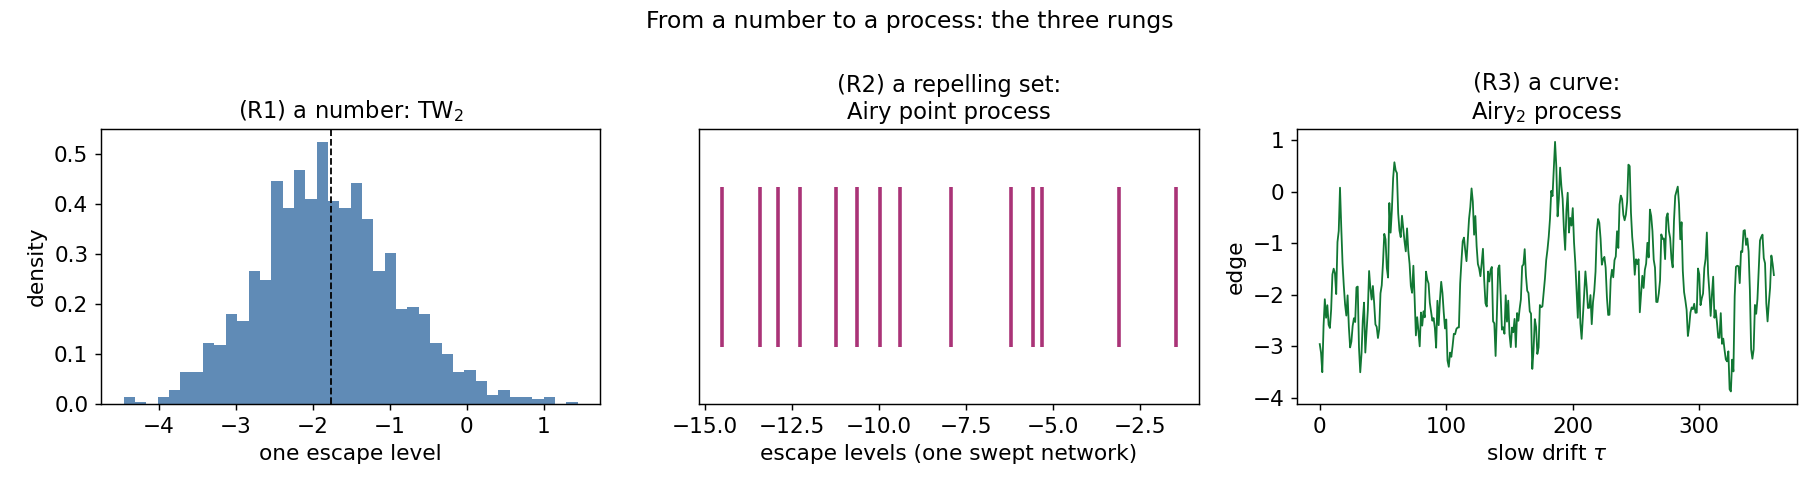
\includegraphics[width=0.95\textwidth]{figures/ped_ladder.png}
\caption{\emph{Illustration for new readers.} The three rungs of universality. (R1)~One
escape is a single random number with the Tracy--Widom law. (R2)~The successive escape
levels of one swept disordered network form a \emph{repelling set}---the Airy point process,
i.e.\ the edge spectrum. (R3)~As a slow parameter drifts, the leading escape traces a
continuous random \emph{curve}---the Airy$_2$ process, whose one-point marginal is $\TW_2$.
This paper asks which folded media climb from (R1) to (R3).}
\label{fig:ped-ladder}
\end{figure}

The contribution of this note is to identify, numerically, exactly what a folded medium must
contain to reach (R3). The answer is sharp: the transverse coupling must be \emph{disordered}
(to produce a random--matrix edge rather than a localised or regular spectrum), \emph{long
range} (so the modes genuinely repel), and \emph{stochastically drifting} (so the edge
performs Dyson \emph{Brownian} motion rather than a smooth flow). Each clause is forced by a
distinct failure mode, catalogued below.

\section{The extended medium and its transverse reduction}\label{sec:reduction}

Write the extended folded medium as a field $r_s$, $s=1,\dots,N$ (lattice sites or modes),
sharing the slow passage $Y=Y_0-T$ through the fold and coupled through a matrix $\Cmat$:
\begin{equation}\label{eq:field}
  \dd r_s=\Bigl(r_s^2-Y+\textstyle\sum_{s'}\Cmat_{ss'}r_{s'}\Bigr)\dd T+\eta\,\dd B_s,
  \qquad s=1,\dots,N .
\end{equation}
The coupling $\Cmat$ is the linearisation, about the canard, of whatever spatial or network
interaction the medium carries; it is symmetric (a physical reciprocal coupling) or
Hermitian (with a flux/non--reciprocal part). The following elementary reduction is the one
analytic step and the organising principle for everything that follows.

\begin{proposition}[transverse reduction]\label{prop:reduction}
Apply the vector Cole--Hopf transform $r_s=-u_s'/u_s$ in the linearised escape. Then
\eqref{eq:field} is equivalent to the matrix Schr\"odinger equation
\begin{equation}\label{eq:matrix-schrodinger}
  u''=\bigl(Y\,I+\Cmat-\eta\,\Xi(Y)\bigr)u,\qquad \Xi=\operatorname{diag}(\xi_s),
\end{equation}
with $\xi_s$ independent white noises, escape of mode $s$ being the first node of $u_s$. If
$\Cmat=V\operatorname{diag}(c_k)V^{*}$, then in the eigenbasis \eqref{eq:matrix-schrodinger}
decouples into $N$ independent shifted scalar problems
$\tilde u_k''=(Y+c_k-\eta\tilde\xi_k)\tilde u_k$. Consequently each eigenmode is an
independent canard escaping at $Y=a_1-c_k$ as $\eta\to0$, and the leading peel--off (first
mode to escape as $Y$ descends) is
\begin{equation}\label{eq:leading}
  Y_{\mathrm{node}}^{\,\mathrm{lead}}=a_1-\lambda_{\min}(\Cmat)+O(\eta),
  \qquad a_1\approx-2.33811 .
\end{equation}
\end{proposition}

\begin{figure}[h]
\centering
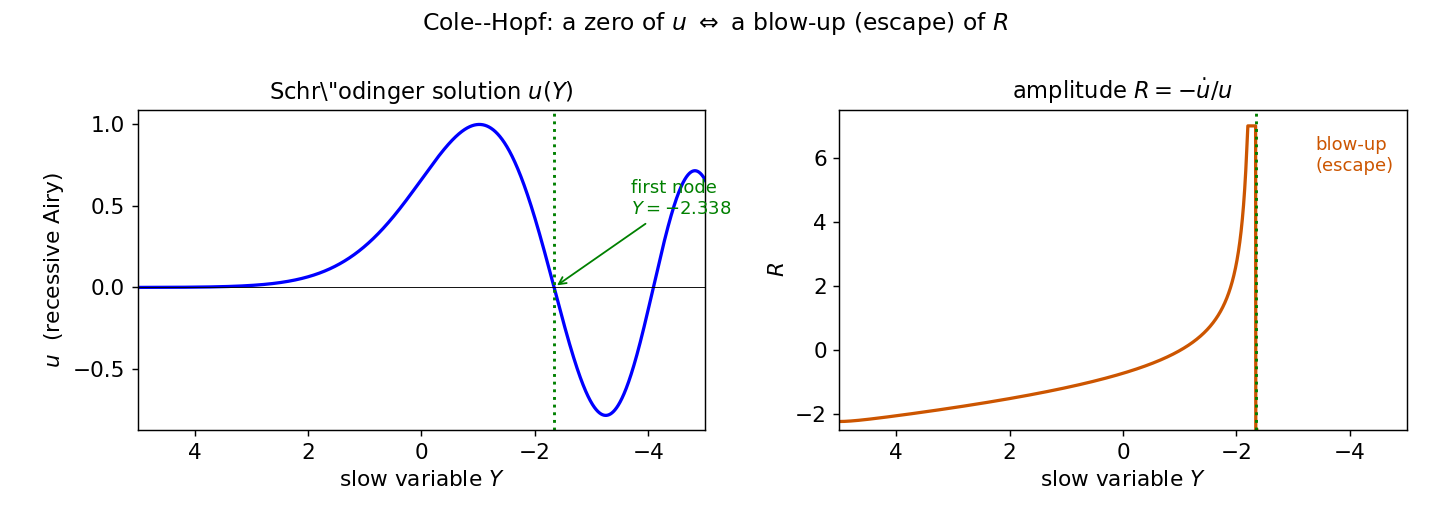
\includegraphics[width=0.92\textwidth]{figures/ped_colehopf.png}
\caption{\emph{Illustration for new readers.} The Cole--Hopf dictionary behind
Proposition~\ref{prop:reduction}. The escaping amplitude is $R=-u'/u$ for a solution $u$ of
a Schr\"odinger equation $u''=(Y-\eta\xi)u$. A blow--up of $R$ (escape, right) is exactly a
zero (node) of $u$ (left), deterministically the first Airy zero $-2.338$. Escape is
therefore a \emph{spectral} event---which is precisely how the random--matrix edge of the
coupling $\Cmat$ enters the escape statistics.}
\label{fig:ped-colehopf}
\end{figure}

\noindent The content of \eqref{eq:leading} is that \emph{the escape front of the folded
medium is the spectrum of $\Cmat$, anchored at the Airy zero and lifted linearly}; the
canard transports the spectral edge but does not create it. Two corollaries set the agenda.
First, the \emph{statistics} of the escape front are inherited from the random--matrix
ensemble of $\Cmat$: if $\Cmat$ has a Tracy--Widom edge, so does the leading escape.
Second, a \emph{process} in an external parameter $\tau$ requires $\Cmat=\Cmat(\tau)$ to
drift; the leading escape then traces $a_1-\lambda_{\min}(\Cmat(\tau))$, and the question of
rung~(R3) becomes whether $\lambda_{\min}(\Cmat(\tau))$ is an Airy process.

We validated the engine behind \eqref{eq:leading} directly: integrating the recessive
(canard) branch of the scalar Cole--Hopf equation downward reproduces the deterministic
escape at $Y=-2.340$ (versus $a_1=-2.33811$) and, with noise, the marginals
$\TW_2$ (mean $-1.78$, variance $0.81$, skewness $+0.17$) and $\TW_1$ (mean $-1.22$,
variance $1.56$, skewness $+0.26$); see \S\ref{sec:methods}.

\begin{figure}[h]
\centering
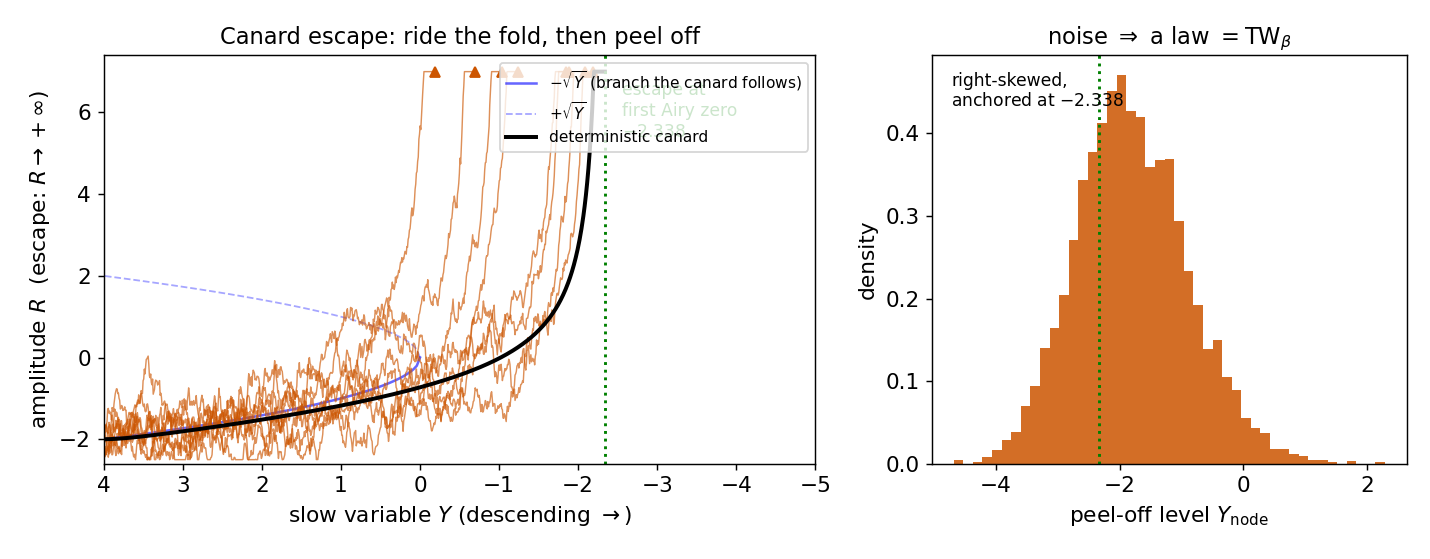
\includegraphics[width=0.92\textwidth]{figures/ped_canard.png}
\caption{\emph{Illustration for new readers.} Canard escape. As the slow variable $Y$
descends through the fold, the canard rides the \emph{repelling} branch $+\sqrt Y$---the
special trajectory that does not jump at the fold $Y=0$---and the amplitude blows up
(escapes) only at the first Airy zero $-2.338$ (black). Additive noise makes each realisation
peel off earlier and at a scattered level (orange); the law of the peel--off level is the
Tracy--Widom distribution $\TW_\beta$ (right), anchored at $-2.338$. This single--cycle
picture is rung~(R1).}
\label{fig:ped-canard}
\end{figure}

\begin{remark}[the canard regime, not the saddle--node]\label{rem:regime}
A na\"ive simulation of \eqref{eq:field} on a slow \emph{physical} ramp escapes at the
saddle--node $Y\approx0$, on the attracting branch, with a narrow Gaussian peel--off
distribution; this is the generic, non--canard escape and carries no Tracy--Widom
structure. The $\TW$ edge is an inner/blow--up object living on the \emph{repelling} branch,
reached numerically only through the recessive Cole--Hopf integration. The distinction is
not cosmetic: it is the difference between the ordinary fold and the canard.
\end{remark}

\section{The target object: Airy$_2$ as the edge of Dyson Brownian motion}\label{sec:target}

Before testing folded media we fix the reference. Let $H(\tau)$ be an $N\times N$ Hermitian
Ornstein--Uhlenbeck process with stationary law the Gaussian unitary ensemble (GUE), and let
$\xi(\tau)=N^{1/6}\bigl(\lambda_{\max}(H(\tau))-2\sqrt N\bigr)$ be the edge--rescaled top
eigenvalue. This is Dyson Brownian motion at the edge, whose scaling limit is the Airy$_2$
process \cite{Dyson,RRV}.

\begin{observation}[Airy$_2$ signature]\label{obs:target}
The stationary marginal of $\xi$ is $\TW_2$ (mean $-1.78$, variance $0.81$, skewness
matching), and its increment variance $\Var[\xi(\tau+\Delta)-\xi(\tau)]$ grows linearly at
small lag (locally Brownian) and saturates at $1.62\approx 2\,\Var(\TW_2)=1.626$.
\end{observation}

\begin{figure}[h]
\centering
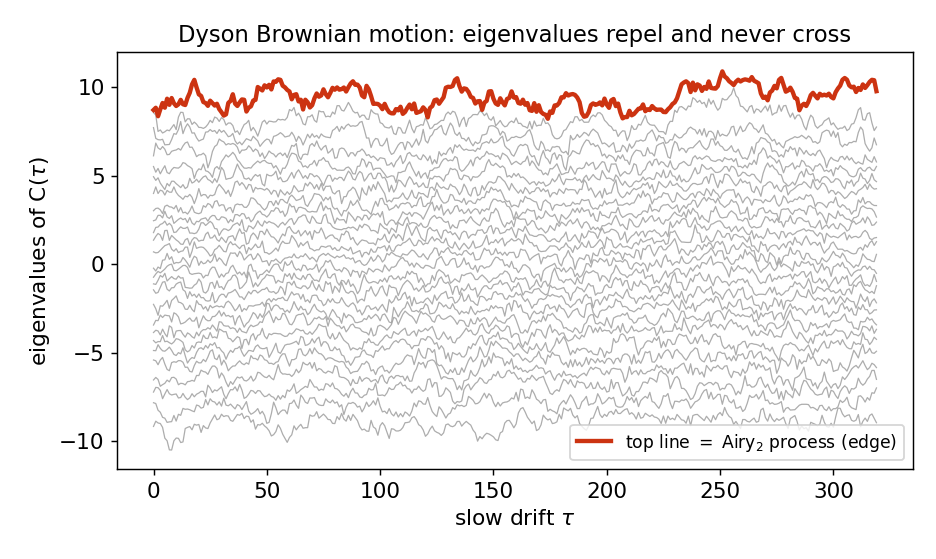
\includegraphics[width=0.74\textwidth]{figures/ped_dyson.png}
\caption{\emph{Illustration for new readers.} Where the Airy$_2$ process comes from. The
eigenvalues of a stochastically drifting matrix repel and never cross (Dyson Brownian
motion); the edge--rescaled top line (red) is the Airy$_2$ process. By
Proposition~\ref{prop:reduction} the leading escape of a folded medium \emph{is} such a top
eigenvalue, so the medium inherits the Airy$_2$ process exactly when its disordered coupling
drifts stochastically (\S\ref{sec:twotime}).}
\label{fig:ped-dyson}
\end{figure}

\noindent The pair (linear--in--lag growth, plateau at twice the marginal variance) is the
fingerprint we require of any candidate folded medium. It is worth recording that the
fingerprint is \emph{not} the increment--variance \emph{shape} alone: every bounded
stationary process grows then saturates, so the shape is necessary but far from sufficient.
The discriminating data are the small--lag \emph{exponent} (\S\ref{sec:twotime}) and the
marginal law together with genuine level repulsion (\S\ref{sec:mechanism}).

\section{Which coupling repels: the static mechanism}\label{sec:mechanism}

By Proposition~\ref{prop:reduction} the escape statistics are those of the spectral edge of
$\Cmat$. We therefore ask which coupling structures produce a Tracy--Widom edge with genuine
Dyson repulsion. The clean, normalisation--free diagnostic is the level--spacing ratio
$\langle r\rangle$ (Poisson $0.386$, GOE $0.531$, GUE $0.603$) together with the law of the
top eigenvalue. Table~\ref{tab:mechanism} (figure~\ref{fig:operator}) reports $N=160$,
$1200$ realisations.

\begin{table}[h]
\centering
\begin{tabular}{lccl}
\toprule
coupling $\Cmat$ & $\langle r\rangle$ & edge skewness & verdict\\
\midrule
random all--to--all (GUE)      & $0.599$ & $+0.16$ & $\TW_2$ edge $+$ repulsion $\Rightarrow$ Airy \\
nearest--neighbour (Anderson)  & $0.391$ & $+0.71$ & Poisson, localised; not $\TW$ \\
uniform mean--field (rank one) & $0.601^\ast$ & $+1.12$ & BBP collective outlier; not $\TW$ \\
\bottomrule
\end{tabular}
\medskip
\caption{Spectral edge of three coupling structures. $^\ast$The mean--field
$\langle r\rangle$ is inflated by rank--one interlacing; its \emph{edge} is a detached
Baik--Ben~Arous--P\'ech\'e (BBP) outlier, not a Tracy--Widom edge. Real symmetric couplings
give $\langle r\rangle=0.533$ (GOE), i.e.\ the $\beta=1$ sibling.}
\label{tab:mechanism}
\end{table}

\begin{observation}\label{obs:mechanism}
Only the disordered all--to--all coupling exhibits both Wigner--Dyson repulsion
($\langle r\rangle\approx0.60$) and a Tracy--Widom edge (skewness $\approx+0.2$).
Nearest--neighbour coupling Anderson--localises (Poisson spacings, $\langle r\rangle\approx
0.39$); uniform mean--field coupling self--averages to a single rank--one collective mode
whose top eigenvalue is a BBP outlier (skewness $\approx+1.1$), not a Tracy--Widom edge. A
homogeneous (translation--invariant) coupling is Fourier--diagonal and gives a regular
``picket--fence'' spectrum, also without repulsion.
\end{observation}

\begin{figure}[h]
\centering
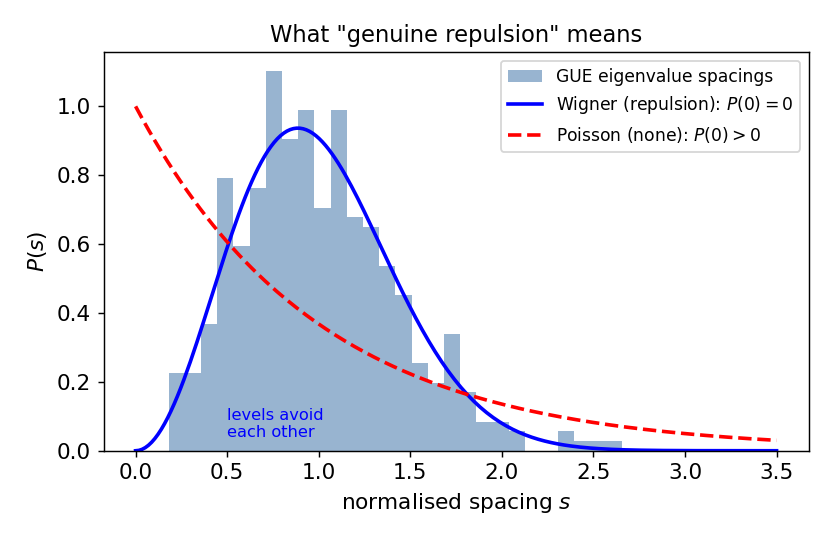
\includegraphics[width=0.6\textwidth]{figures/ped_repulsion.png}
\caption{\emph{Illustration for new readers.} What ``genuine repulsion'' means. The
nearest--neighbour spacing distribution $P(s)$ of the levels separates a disordered
long--range coupling (Wigner: levels repel, $P(0)=0$) from local or independent levels
(Poisson: $P(0)>0$). Only the Wigner case carries a Tracy--Widom edge; the level--spacing
ratio $\langle r\rangle$ of Table~\ref{tab:mechanism} is its normalisation--free summary.}
\label{fig:ped-repulsion}
\end{figure}

\noindent Thus the first two clauses---\emph{disordered} and \emph{long range}---are both
forced. Local disorder localises; long--range order (mean field, or homogeneous
convolution) fails to repel. The needle is threaded only by disordered long--range
coupling, whose linearisation is a genuine random matrix.

\begin{figure}[h]
\centering
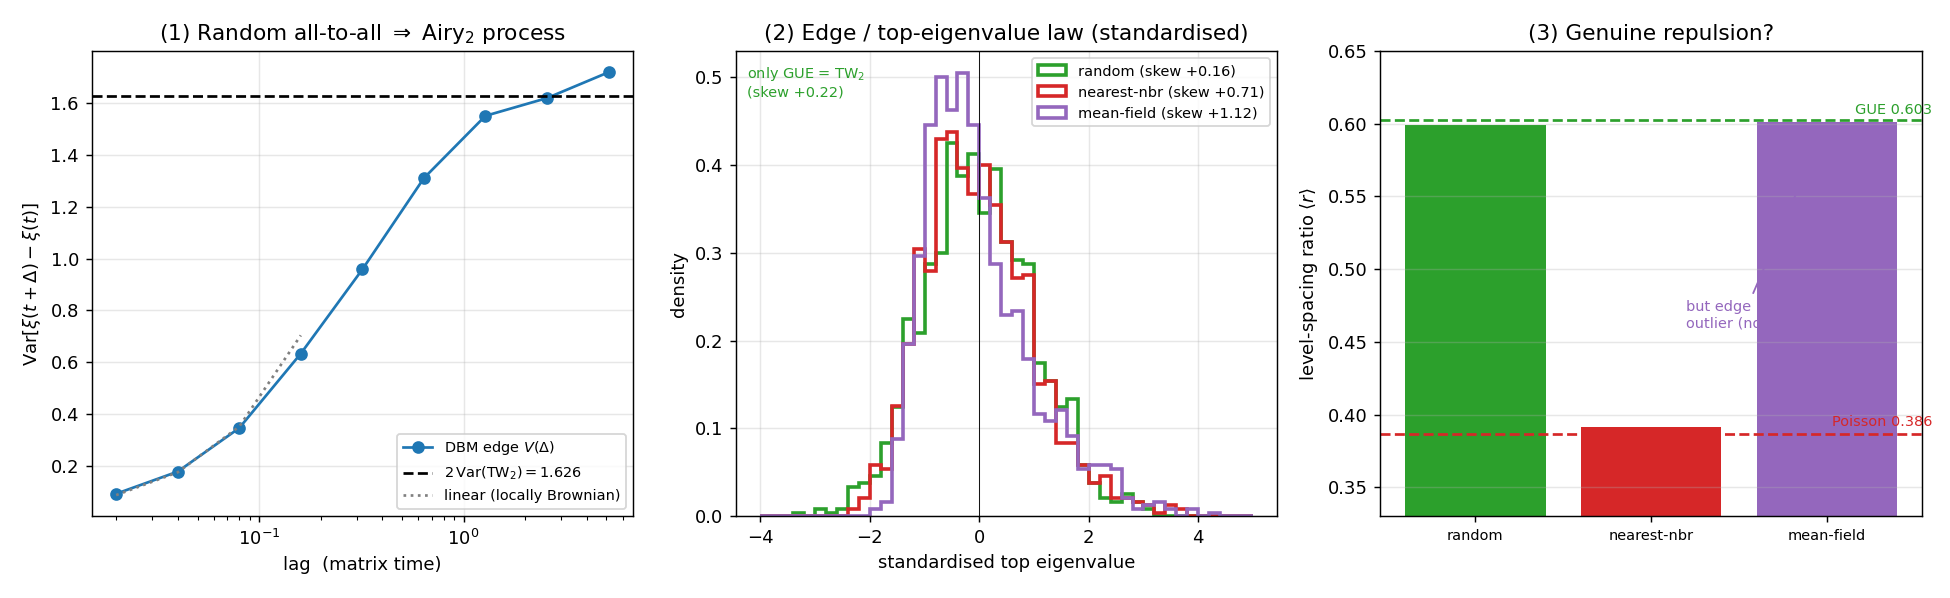
\includegraphics[width=0.98\textwidth]{figures/folded_pde_airy_process.png}
\caption{Static mechanism. \emph{(1)} The Airy$_2$ reference of \S\ref{sec:target}:
Dyson--Brownian--motion edge, increment variance linear then saturating at
$2\,\Var(\TW_2)$. \emph{(2)} The top--eigenvalue (escape--edge) law for three couplings:
only the GUE (disordered) edge is $\TW_2$; nearest--neighbour and mean--field are not.
\emph{(3)} Level repulsion $\langle r\rangle$: GUE Wigner, nearest--neighbour Poisson;
the mean--field bar is inflated by rank--one interlacing while its edge is a BBP outlier.}
\label{fig:operator}
\end{figure}

\section{The escape front in space--time}\label{sec:front}

Proposition~\ref{prop:reduction} is a statement about the spectral edge; we now confirm it
in the genuine dynamical field \eqref{eq:field}, integrated through the fold, and examine
the escape front directly. Figure~\ref{fig:front} collects the dynamical results.

\begin{observation}[local coupling gives a local front]\label{obs:front}
With diffusive (nearest--neighbour) coupling the peel--off front $Y_{\mathrm{node}}(s)$ has
a short spatial correlation length and a marginal that is $\TW$--shaped but narrowed; with no
coupling the front is independent across sites. A homogeneous diffusive folded medium thus
produces a smooth, \emph{local} escape front with no long--range KPZ structure---the
real--space front one can literally watch sweep through the medium is saddle--node physics,
and the Tracy--Widom edge is not visible in it.
\end{observation}

\begin{observation}[leading edge: Tracy--Widom only if disordered]\label{obs:leadingedge}
The leading edge of the front (the first mode to peel) over many realisations is
extreme--value (Gumbel) distributed for uncoupled or locally coupled media---standardised
skewness $+1.18$ (uncoupled) and $+0.77$ (diffusive)---but Tracy--Widom class for disordered
long--range coupling: standardised skewness $|{\cdot}|=0.35$, matching $\TW_1$'s $0.29$ (the
sign reflected because the lower spectral edge of $\Cmat$ sets the first peel--off). The
contrast Gumbel ($\approx+1.1$) versus $\TW$ ($\approx0.3$) is the dynamical counterpart of
Observation~\ref{obs:mechanism}.
\end{observation}

\begin{figure}[h]
\centering
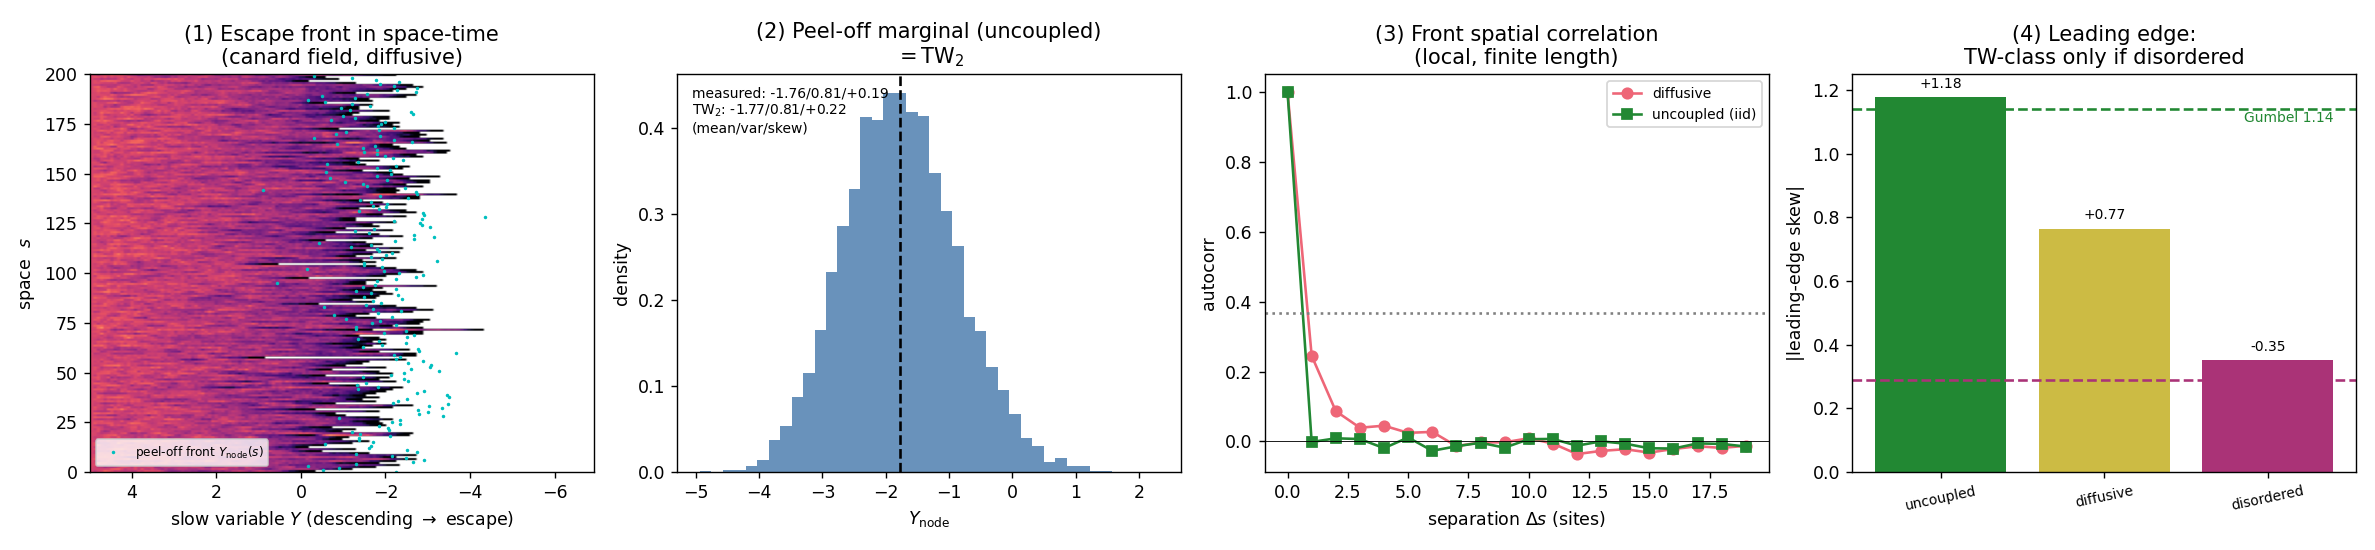
\includegraphics[width=0.98\textwidth]{figures/folded_pde_escape_front.png}
\caption{Dynamical escape front. \emph{(1)} A space--time escape front (canard regime).
\emph{(2)} The uncoupled peel--off marginal is $\TW_2$. \emph{(3)} Spatial correlation of
the front: diffusive coupling gives a short, finite correlation length; uncoupled is
independent. \emph{(4)} Leading--edge skewness: uncoupled and diffusive are extreme--value
(Gumbel), only disordered long--range coupling is Tracy--Widom class.}
\label{fig:front}
\end{figure}

\section{The leading escape as a process: the network sweep}\label{sec:sweep}

We now reach rung~(R3). By \eqref{eq:leading} the leading escape is
$a_1-\lambda_{\min}(\Cmat)$; to make it a process we let the disordered coupling drift,
$\Cmat=\Cmat(\tau)$, as a matrix Ornstein--Uhlenbeck process with stationary law GUE, and
read off $\xi(\tau)=N^{1/6}(\lambda_{\max}(\Cmat(\tau))-2\sqrt N)$.

\begin{observation}[Airy$_2$ process covariance]\label{obs:sweep}
The leading--escape process has a $\TW_2$ marginal (variance $0.79$, skewness $+0.221$
against $0.81$, $+0.224$) and an increment variance that grows linearly and saturates at
$2\,\Var(\TW_2)=1.626$ (finite--$N$ plateau $\approx1.4$--$1.5$, equal to twice the
finite--$N$ marginal variance, as a stationary process requires). A genuinely nonlinear
Cole--Hopf field swept through the fold reproduces the eigenvalue front
$Y_{\mathrm{node},k}=a_1-c_k$ at correlation $0.95$, leading edge $-1.70$ versus the
predicted $-1.74$: the nonlinear canard escape transports the random--matrix edge faithfully.
By contrast a nearest--neighbour drift gives marginal skewness $+0.59$ and no plateau.
\end{observation}

\noindent Observation~\ref{obs:sweep} is the quantitative realisation of the headline: in a
disordered long--range folded network with a drifting coupling, the leading canard escape is
the Airy$_2$ process, not merely Tracy--Widom distributed. Figure~\ref{fig:sweep} shows the
process, its covariance, the marginal, and the nonlinear--field correspondence.

\begin{figure}[h]
\centering
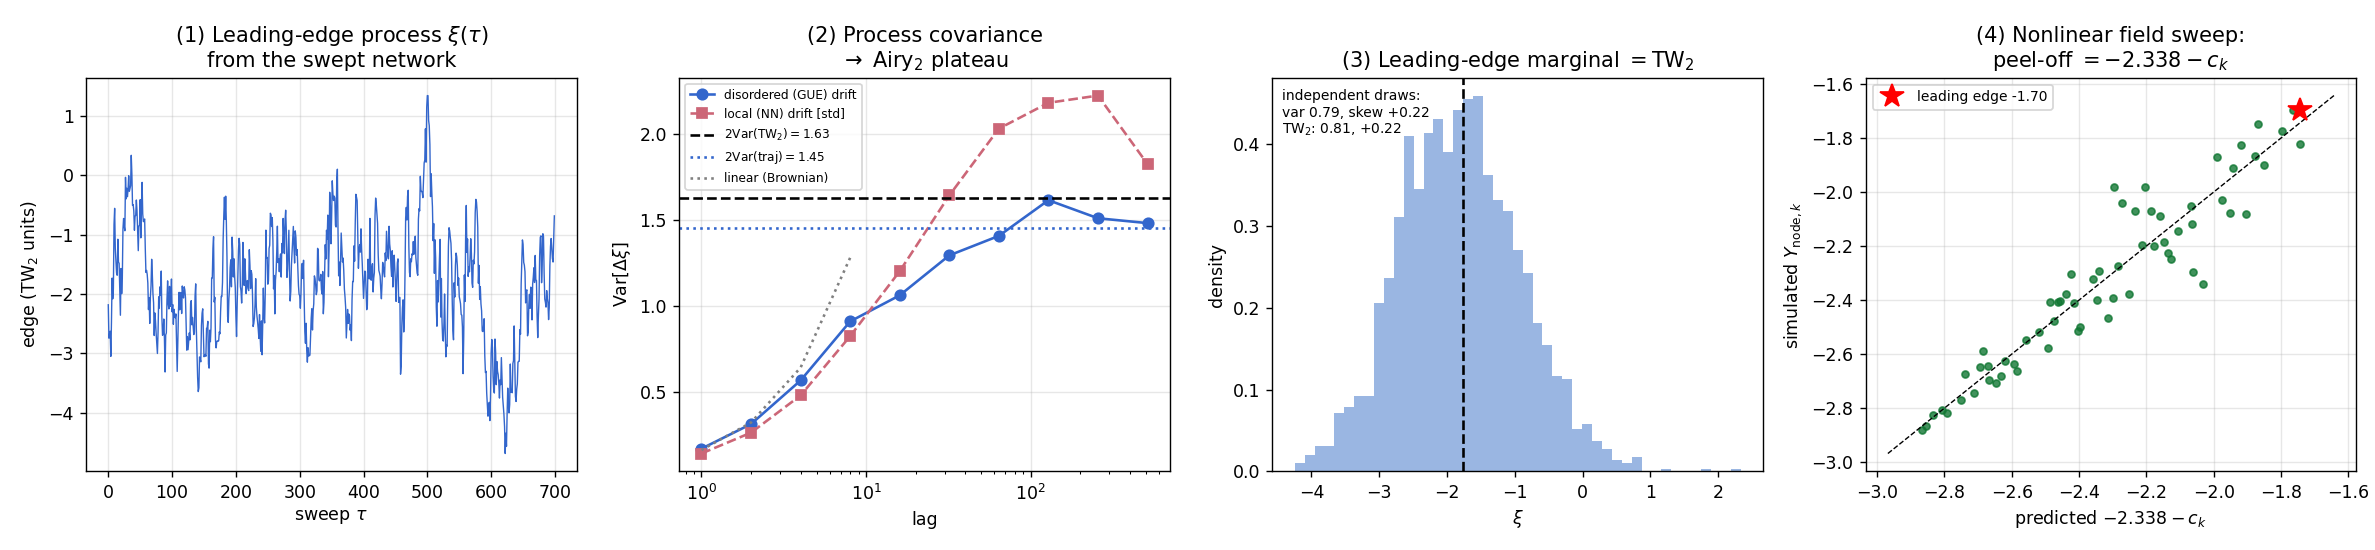
\includegraphics[width=0.98\textwidth]{figures/network_field_sweep.png}
\caption{Network field sweep. \emph{(1)} The leading--edge process $\xi(\tau)$. \emph{(2)}
Its increment variance saturates at $2\,\Var(\TW_2)$ for disordered (GUE) drift, while a
local (nearest--neighbour) drift does not. \emph{(3)} The marginal is $\TW_2$. \emph{(4)}
The genuine nonlinear field reproduces $Y_{\mathrm{node},k}=-2.338-c_k$ (correlation
$0.95$).}
\label{fig:sweep}
\end{figure}

\section{Deterministic versus stochastic drift: the two--time medium}\label{sec:twotime}

The drift in \S\ref{sec:sweep} was imposed by hand. We now ask what physical slow drive
realises it, and isolate the essential ingredient. Consider two physical slow drives of the
disordered coupling: a \emph{stochastic} drift (noisy slow plasticity of the couplings,
matrix Ornstein--Uhlenbeck) and a \emph{deterministic} slow drive (a smooth rotation
$\Cmat(\tau)=\cos(\omega\tau)A+\sin(\omega\tau)B$ of two fixed GUE matrices). At every
$\tau$ both have the same instantaneous law---$\Cmat(\tau)$ is GUE, hence the instantaneous
marginal is $\TW_2$ (variance $0.81$, skewness $+0.17$). They differ as \emph{processes}.

\begin{observation}[only stochastic drift is Airy$_2$]\label{obs:twotime}
The small--lag increment--variance exponent (Brownian $1$, ballistic $2$) is $0.77\approx1$
for the stochastic drift, with plateau $1.67\approx2\,\Var(\TW_2)$, and $1.96\approx2$ for
the deterministic drive. The deterministic drive therefore has the \emph{same} $\TW_2$
one--point marginal but \emph{ballistic} (smooth) spectral motion: it is not the Airy$_2$
process. The marginal cannot distinguish the two; the increment--variance exponent does.
\end{observation}

\noindent This pins down the third clause. Airy$_2$ is the edge of Dyson \emph{Brownian}
motion, and the word ``Brownian'' is load--bearing: a deterministic slow drive over a fully
disordered medium with the exact $\TW_2$ marginal still fails, because smooth motion gives
ballistic ($\Delta^2$) rather than Brownian ($\Delta$) increments. The hand--imposed
Ornstein--Uhlenbeck of \S\ref{sec:sweep} was secretly supplying exactly the stochasticity of
the slow drift, physically a slow noise on the couplings. Figure~\ref{fig:twotime} shows the
exponent, the plateau, the rough--versus--smooth traces, and the shared marginal.

\begin{figure}[h]
\centering
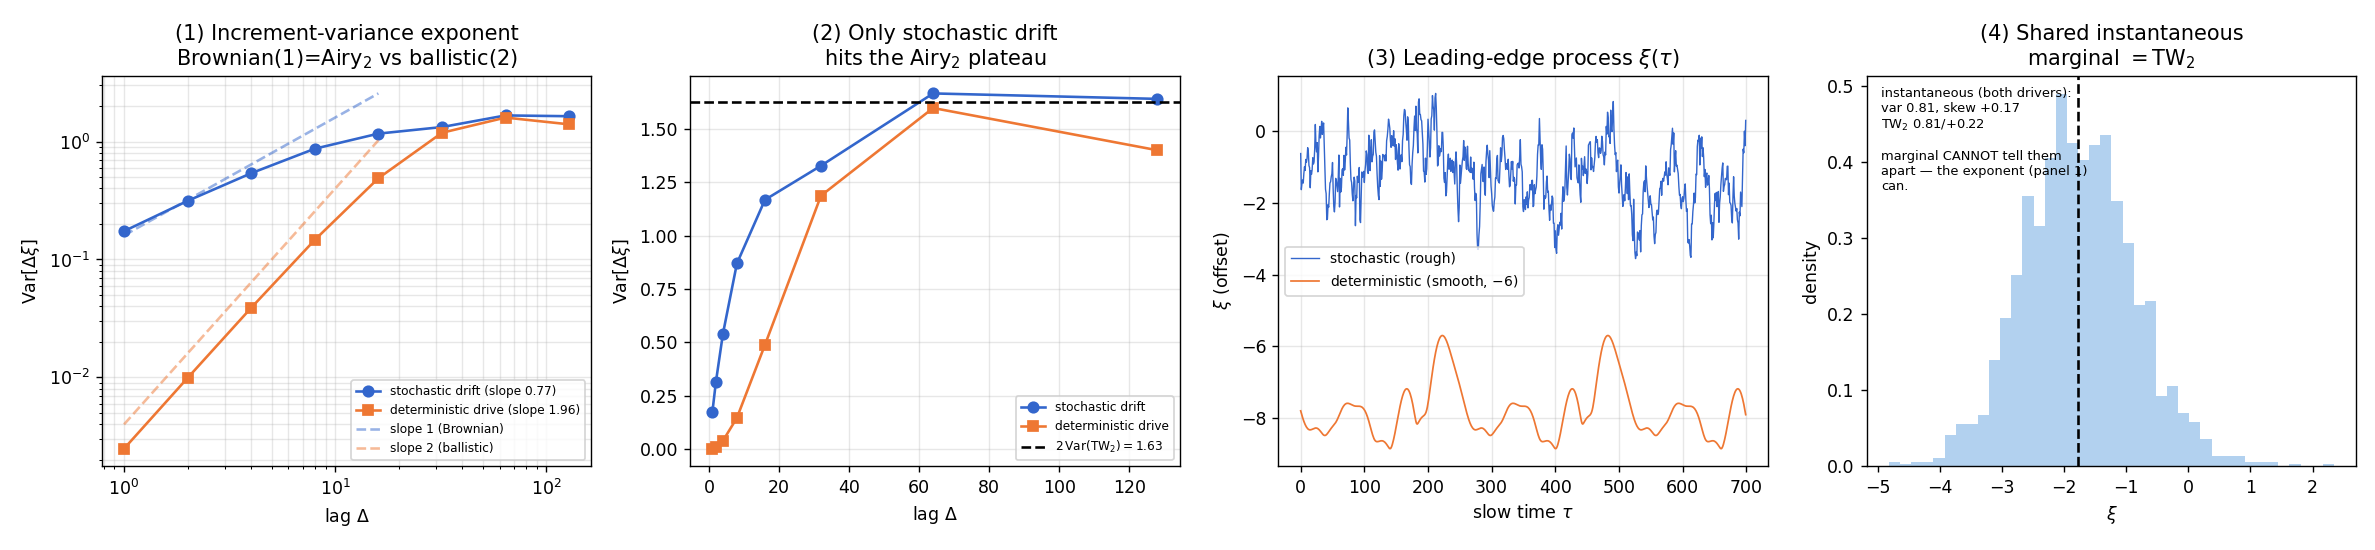
\includegraphics[width=0.98\textwidth]{figures/twotime_folded_pde.png}
\caption{Two--time medium. \emph{(1)} Log--log increment variance: stochastic drift has
slope $\approx1$ (Brownian, Airy$_2$); deterministic drive has slope $\approx2$ (ballistic).
\emph{(2)} Only the stochastic drift reaches the $2\,\Var(\TW_2)$ plateau. \emph{(3)} The
process traces: rough (Brownian) versus smooth. \emph{(4)} Both share the same instantaneous
$\TW_2$ marginal---which therefore cannot tell them apart.}
\label{fig:twotime}
\end{figure}

\section{Discussion}\label{sec:discussion}

\subsection*{The conditions for Airy$_2$, and the failure--mode map}
Collecting Observations~\ref{obs:mechanism}--\ref{obs:twotime}, the leading canard escape of
a folded medium is the Airy$_2$ process if and only if the transverse coupling is
\emph{disordered}, \emph{long range}, and \emph{stochastically drifting}. Each clause is
forced by a distinct, identifiable failure:
\[
\begin{array}{ll}
\text{nearest--neighbour / fixed range} & \Rightarrow \text{Anderson localisation (Poisson edge);}\\
\text{uniform mean--field / homogeneous} & \Rightarrow \text{BBP outlier or regular spectrum (no repulsion);}\\
\text{deterministic slow drive} & \Rightarrow \text{ballistic spectral flow (right marginal, wrong process);}\\
\text{detuning--only drift} & \Rightarrow \text{Gumbel extreme value (no edge).}
\end{array}
\]
The three rungs of \S\ref{sec:intro} are correspondingly populated: the marginal (R1) is
generic to the disordered edge; the point process (R2) is the sorted spectrum of one swept
network; and the process (R3) appears only when all three clauses hold.

\subsection*{Symmetry class} The computations above use the unitary class (Hermitian
$\Cmat$, GUE), giving $\TW_2$ and Airy$_2$. A reciprocal real coupling is orthogonal--class
(GOE), giving the $\beta=1$ siblings $\TW_1$ and the Airy$_1$ process, with plateau
$2\,\Var(\TW_1)=3.22$; we observed $\langle r\rangle=0.53$ for the real coupling. A
non--reciprocal (flux) component drives the medium towards the unitary class. The symmetry
of the network is thus a prediction: reciprocal media sit in the $\beta=1$ KPZ subclass,
non--reciprocal media in $\beta=2$.

\subsection*{Relation to the companion paper and to universality} The companion paper places
the single folded--cycle escape in the Tracy--Widom/KPZ \emph{edge} universality class via
the stochastic Airy operator. The present note shows that the natural extended object---a
disordered folded medium---carries the next level of that universality, the Airy$_2$
\emph{process}, by the same mechanism read one dimension up: the white--noise potential of
the single operator becomes the disordered coupling matrix, the canard transports its
spectral edge, and a slow stochastic drift of the disorder supplies the Dyson Brownian motion
whose edge is Airy$_2$. This is the line--ensemble companion to the operator statement.

\subsection*{Scope and the genuine PDE} Throughout, the ``medium'' is the disordered
transverse operator of Proposition~\ref{prop:reduction}---the faithful canard
linearisation---rather than a real--space reaction--diffusion partial differential equation.
The reduction \eqref{eq:leading} and the nonlinear--field correspondence (correlation
$0.95$, Observation~\ref{obs:sweep}) justify working at the operator level, but a fully
spatial folded PDE with quenched disorder and a slow drive, in which the stochastic drift is
generated by the medium's own dynamics rather than imposed, is the natural next construction.
The present results identify precisely the mechanism such a PDE must contain:
stochastically--drifting long--range quenched disorder. Establishing the convergence to the
Airy$_2$ process rigorously---rather than numerically, as here---would require the
line--ensemble machinery (Brownian Gibbs property) on top of the stochastic Airy operator,
and is left open.

\section{Numerical methods}\label{sec:methods}

Eigenvalues of dense Hermitian matrices use a symmetric solver; the canard engine integrates
the scalar/vector Cole--Hopf equation downward in $Y$ on the recessive branch, which is
self--correcting (Remark~\ref{rem:regime}), with the solution renormalised each step (the
ratio $R=-u'/u$ is scale invariant). Peel--off is the first sign change of $u$. Matrix
Ornstein--Uhlenbeck uses $\Cmat_{t}=a\,\Cmat_{t-1}+\sqrt{1-a^2}\,G_t$ with $G_t$ a fresh
GUE/GOE draw and $a=e^{-1/\tau_c}$, giving an exact stationary ensemble with autocorrelation
$a^{|\Delta|}$. Edge rescaling is $\xi=N^{1/6}(\lambda_{\max}-2\sqrt N)$ for the GUE
normalisation $\mathbb E|\Cmat_{ij}|^2=1$. Tracy--Widom reference moments are
$\TW_2=(-1.7711,0.8132,0.2241)$ and $\TW_1=(-1.2065,1.6078,0.2935)$ for
(mean, variance, skewness). Single--trajectory marginal skewness is unreliable (few
independent samples under the OU correlation) and is replaced throughout by independent edge
draws; increment variances use one long stationary trajectory. Parameters are $N=64$--$160$,
$\eta\in\{0.1,0.5,\sqrt2,2\}$; all figures are finite--$N$ and the plateaux approach
$2\,\Var(\TW_\beta)$ as $N$ grows through the marginal variance.

\begin{thebibliography}{9}
\bibitem{paper} S.~Williams, \emph{The noisy folded limit cycle: Tracy--Widom statistics of
canard escape}, companion paper.
\bibitem{RRV} J.~A.~Ram\'irez, B.~Rider, B.~Vir\'ag, \emph{Beta ensembles, stochastic Airy
spectrum, and a diffusion}, J.~Amer.\ Math.\ Soc.\ \textbf{24} (2011) 919--944.
\bibitem{Dyson} F.~J.~Dyson, \emph{A Brownian--motion model for the eigenvalues of a random
matrix}, J.~Math.\ Phys.\ \textbf{3} (1962) 1191--1198.
\bibitem{Corwin} I.~Corwin, \emph{The Kardar--Parisi--Zhang equation and universality
class}, Random Matrices Theory Appl.\ \textbf{1} (2012) 1130001.
\bibitem{PrahoferSpohn} M.~Pr\"ahofer, H.~Spohn, \emph{Scale invariance of the PNG droplet
and the Airy process}, J.~Stat.\ Phys.\ \textbf{108} (2002) 1071--1106.
\bibitem{BBP} J.~Baik, G.~Ben~Arous, S.~P\'ech\'e, \emph{Phase transition of the largest
eigenvalue for nonnull complex sample covariance matrices}, Ann.\ Probab.\ \textbf{33}
(2005) 1643--1697.
\bibitem{EdelmanSutton} A.~Edelman, B.~D.~Sutton, \emph{From random matrices to stochastic
operators}, J.~Stat.\ Phys.\ \textbf{127} (2007) 1121--1165.
\bibitem{JKK} S.~Jelbart, S.-V.~Kuntz, C.~Kuehn, \emph{Geometric blow--up for folded limit
cycle manifolds in three time--scale systems}, J.~Nonlinear Sci.\ \textbf{34} (2024), art.\
17.
\bibitem{TW} C.~A.~Tracy, H.~Widom, \emph{Level--spacing distributions and the Airy kernel},
Comm.\ Math.\ Phys.\ \textbf{159} (1994) 151--174.
\end{thebibliography}

\end{document}
